\section{Approach}
\label{sec:method}
As for each non-question utterance, we extract it with each question from the other participant before it to combine a sample for the model. We also extract the dialogue context information for each pair, including distance and history. Distance refers to the number of utterances between the question and non-question in a sample, and history is made up of the utterances between them. 

Inspired by match-LSTM with word-by-word attention \cite{wang2015learning}, we propose an attention based neural network model for answer assignment in multi-turn dialogues. The neural network model consists of four components: \textbf{Sentence Encoder} transforms the natural language utterances into sentence-level embeddings. \textbf{History Attention} add history information into the pairwise model based on two parallel attention mechanisms. \textbf{Match-LSTM} is used to compare the processed sentence pair word by word. Finally, \textbf{Prediction Layer} bring the distance information into consider and calculate the final alignment probability for the inputs.
 %\textbf{History Adder} consists of two parallel attention mechanisms to add history information into the pairwise model. 

\begin{figure*}
	\centering
	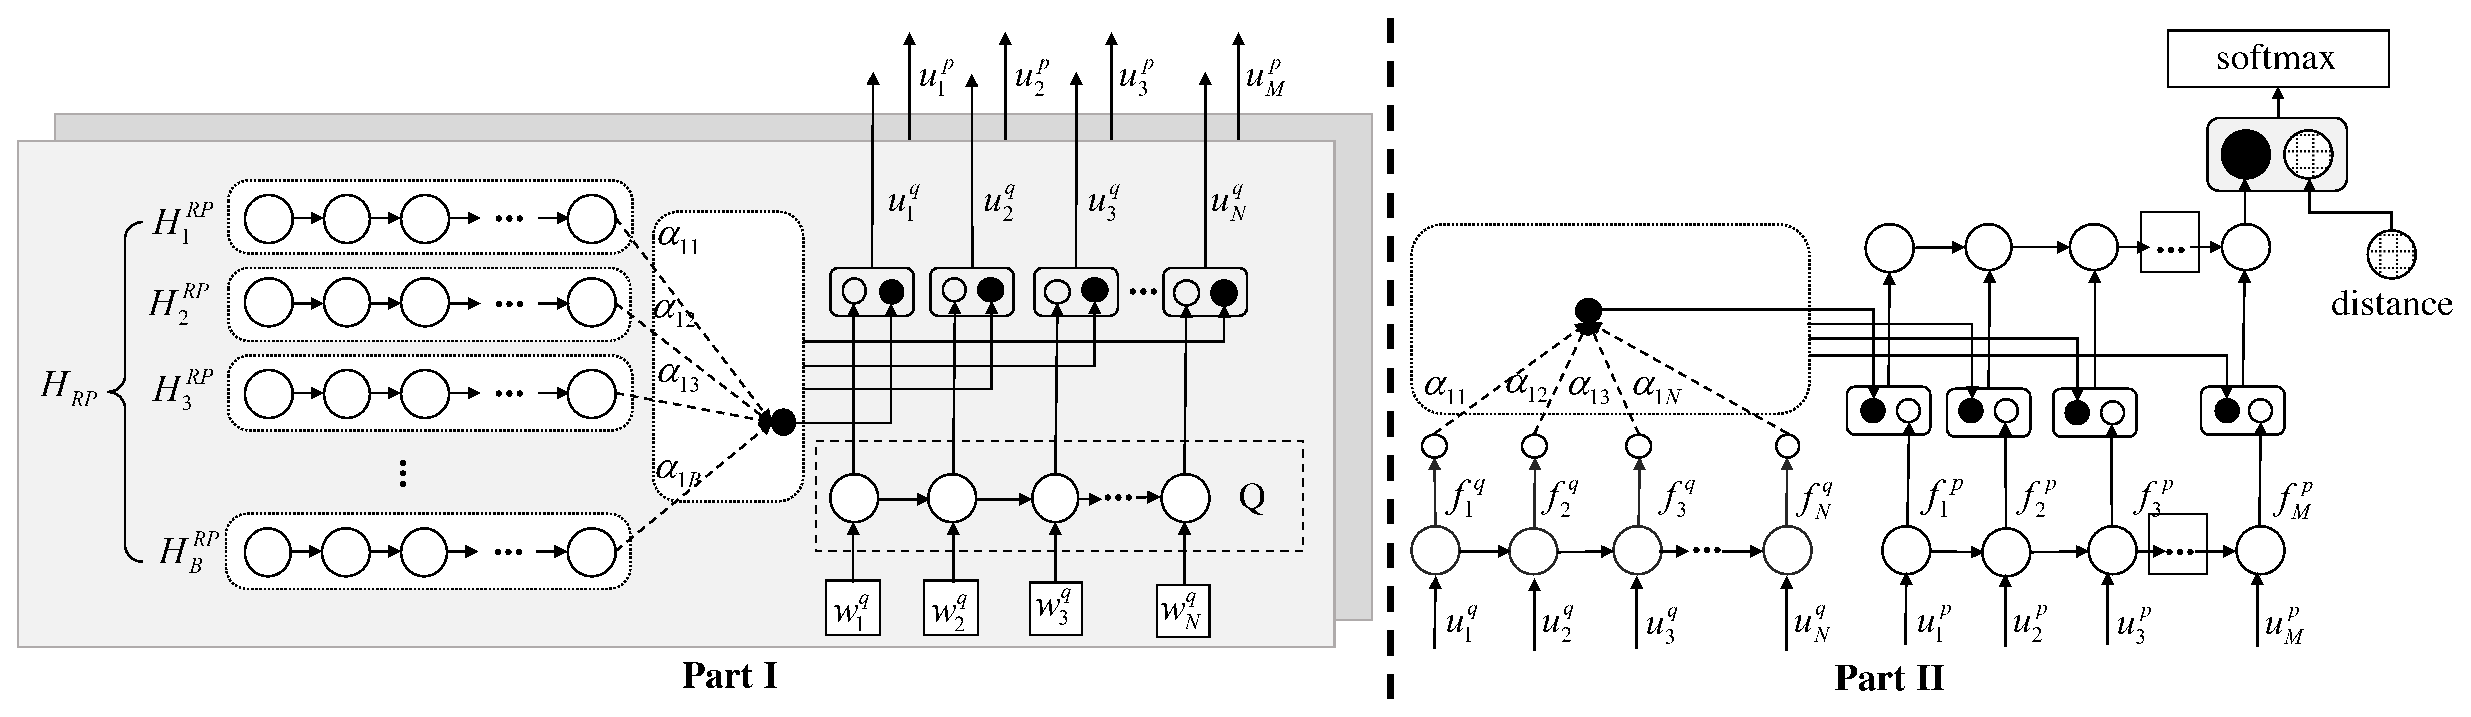
\includegraphics[scale=0.42]{pictures/figure4.eps}
	\caption{The architecture of the proposed match-LSTM based model with parallel attention mechanisms. \textbf{Part I:} History Attention. \textbf{Part II:} Match-LSTM Component}
	
	\label{fig:model1}
\end{figure*}

\subsection{Sentence Encoder}
\label{sec:sentence-encoder}

Consider a Q and an NQ, we first convert the words to their word-level embeddings ($Q=\{w_i^q\}_{t=1}^{N}$ and $NQ= \{w_i^p\}_{t=1}^{M}$) using pretrained word embeddings.

We name the participant who raised the question utterance as $role_Q (RQ)$. The other participant who raised the non-question utterance is named as $role_P (RP)$. After converting each word to embedding, $H_{RQ}=\{ \{w_{1t}^{q}\}_{t=1}^{N_1}, \{w_{2t}^{q}\}_{t=1}^{N_2}... ,\{w_{At}^{q}\}_{t=1}^{N_A} \}$ and $H_{RP}=\{ \{w_{1t}^{p}\}_{t=1}^{M_1}, \{w_{2t}^{p}\}_{t=1}^{M_2}... ,\{w_{Bt}^{p}\}_{t=1}^{M_B} \}$.

 We then use one-layer LSTM model proposed by \cite{gers1999learning} to obtain the sentence embedding. Specifically, we use all the hidden states output from LSTM to encode $Q$ ($\{h_t^q\}_{t=1}^{N}$) and $NQ$ ($ \{h_t^p\}_{t=1}^{M}$), but use the last state of LSTM to encode several history sentences in $H_{RQ}$ ($\{d_t^q\}_{t=1}^{A}$) and $H_{RP}$ ($\{d_t^p\}_{t=1}^{B}$).



\subsection{History Attention}
%To matching QA pairs embed in 
To match IQA pairs and long distance pairs, we consider bringing dialogue history information into the model by using attention mechanisms. We divide the history into two parts: one is contributed by the questioner, and the other by the answerer. Besides, we utilize two parallel attention mechanisms: one for combining $H_{RP}$ into $Q$ and the other for combining $H_{RQ}$ into $NQ$. In this interleaving history adding way, we can get more information about interaction effect between two participants. For example, when dealing with the Q-NQ pair $\{U2,U10\}$, $\{U4,U5,U6,U8\}$ is the history provided by answerer. We combined these history information %selected by $U2$ 
into $U2$, so that the probability of matching far-away broken answer $U10$ with $U2$ will increase since the former part of the answers are considered. As for the Q-NQ pair of $\{U1,U11\}$, all the utterances from $U2$ to $U10$ will be considered in our model, which may increase the probability of labeling such IQA relations.
 %covered
  %out
%while covering the whole history. 
%Mathematically,take a question $Q=[h^q_1,h^q_2,...,h^q_N]$ and the history $H_{RP}=\{d^p_1,d^p_2,...,d^p_B\}$ as an example. Borrowing idea from \cite{wang2015learning} and \cite{rocktaschel2015reasoning}, the question containing historical information via soft alignment of words in the question and sentences in the history can be obtained as follows:

Borrowing idea from Wang et al.~\shortcite{wang2017gated}, the question containing historical information via soft alignment of words in the question $Q=[h^q_1,h^q_2,...,h^q_N]$ and history sentences $H_{RP}=\{d^p_1,d^p_2,...,d^p_B\}$ can be obtained as follows (see Part I in Figure \ref{fig:model1}):

\begin{equation}
    u^q_t=[h^q_t,c^q_t]
\end{equation}
where $c^q_t=att(h^q_t,H_{RP})$ is an attention pooling vector of the whole history($H_{RP}$):
\begin{equation}
\begin{aligned}
s^t_j&=v^Ttanh(W_Qh^q_t+W_Hd^p_j)\\
a^t_i&=exp(s^t_i)/\sum_{j=1}^Bexp(s^t_j)\\
c^q_t&=\sum_{i=1}^Ba^t_id^p_i
\end{aligned}
\end{equation}
Each word representation in $Q$ dynamically incorporates aggregated matching information from the history $H_{RP}$.

Finally, we get the question and non-question as  $Q=[u^q_1,u^q_2,...,u^q_N]$ and $NQ=[u^p_1,u^p_2,...,u^p_M]$. Each word representation for both utterance not only represent the sentence meaning but also contain dialogue context.



\subsection{Match-LSTM}
We follow the work of Wang and Jiang~\shortcite{wang2015learning} and adopt match-LSTM to find relations between the processed $Q$ and $NQ$ word by word.

Again, we use the LSTM model mentioned in section \ref{sec:sentence-encoder} to encode the processed representations for question and non-question again. Then, we get $Q=\{f^q_t\}_{t=1}^{N}$ and $NQ=\{f^p_t\}_{t=1}^{M}$. When looking through the non-question, we introduce a series of attention-weighted combinations of the hidden states of the question, where each combination is for a particular word in the non-question. The sentence-pair representation $P=\{p_t\}_{t=1}^{M}$ is calculated with attention mechanism as follows (see Part II in Figure \ref{fig:model1}):

\begin{equation}
    p_t=LSTM(p_{t-1},[f^p_t,c_t])
\end{equation}
where $c_t=att(Q,f^p_t,p_{t-1})$ is an attention pooling vector of the whole question($Q$):
%\begin{center}
\begin{equation}
\begin{aligned}
s^t_j&=v^Ttanh(W_{NQ}f^p_t+W_Qf^q_j+W_pp_{t-1})\\
a^t_i&=exp(s^t_i)/\sum_{j=1}^Nexp(s^t_j)\\
c_t&=\sum_{i=1}^Na^t_if^q_i
\end{aligned}
%\end{gather}
\end{equation}
%\end{center}

Finally, we use $p_M$ to represent the whole pair which is used for predicting the final result.

\subsection{Prediction Layer }
At the last step, we use a fully-connected (FC) layer with softmax to do binary classification, which indicates whether this pair of utterance has QA relation.

Besides the final representation $p_M$, we introduce a vector of distance information $d$ to the model. Final probability is calculated as follows:
\begin{equation}
\begin{aligned}
FC&=W[p_M,d]+b\\
Probability&=Softmax(FC)
\end{aligned}
\end{equation}

For a NQ, it has a matching probability with each Q before it. We choose the $Q_{i}$ with the max probability $p$, if $p>0.5$, then we say there is a QA relation between this NQ and associated $Q_{i}$, and this NQ will be labeled as $A_i$. Otherwise, the NQ will be predicted as $O$. 

%For a NQ, it has a matching probability with each Q before it. We first choose the one with the max probability. If the probability surpass the threthold=0.5, then we say there is a QA relation between this Q-NQ pair, and the NQ will be named after $Q_i$ as $A_i$. Otherwise, this NQ will be finally predicted as an O.





